\documentclass{article}
\usepackage{microtype}
\usepackage{graphicx}
\usepackage{booktabs}
\usepackage{hyperref}
\usepackage{icml2026}
\usepackage{amsmath,amssymb,mathtools,amsthm}
\usepackage[capitalize,noabbrev]{cleveref}
\theoremstyle{plain}
\newtheorem{proposition}{Proposition}
\theoremstyle{definition}
\newtheorem{definition}{Definition}
\newtheorem{assumption}{Assumption}
\theoremstyle{remark}
\newtheorem{remark}{Remark}
\newcommand{\Bst}{B^{\ast}}
\newcommand{\Pst}{P^{\ast}}
\newcommand{\Dst}{D^{\ast}}
\newcommand{\rank}{\mathrm{rk}}
\icmltitlerunning{Targeted investment needed to top a multi-task leaderboard}

\begin{document}
\twocolumn[
  \icmltitle{How Much Targeted Training Does It Take to Top a Multi-Task Leaderboard?\\ The Aggregation Rule Sets the Currency of the Investment}
  \begin{icmlauthorlist}
    \icmlauthor{Anonymous Authors}{anon}
  \end{icmlauthorlist}
  \icmlaffiliation{anon}{Anonymous Institution}
  \icmlcorrespondingauthor{Anonymous Authors}{anonymous@example.org}
  \icmlkeywords{benchmarks, leaderboards, aggregation, social choice, evaluation}
  \vskip 0.3in
]
\printAffiliationsAndNotice{}

\begin{abstract}
A multi-task leaderboard ranks models by aggregating per-task scores, so a developer can try to raise one model's rank by training on data related to selected sub-datasets.
We ask what such \emph{targeted investment} must look like for a target model to reach first place, and how this depends on the aggregation rule.
We define investment by three exact measures---the number of tasks touched (breadth $B$), the total score gain ($P$), and the number of test-equivalent questions that must be learned ($D$)---under explicit assumptions (no spillover, static rivals, linear cost, per-task ceilings).
We give closed forms for the mean and for order statistics such as the median, lower bounds for Borda, plurality and Condorcet-type rules (tight for Borda and Condorcet on the data), and solve every case exactly by integer programming on public data: HELM MMLU (79 models, 57 subjects) and the Open LLM Leaderboard (4{,}576 models, 6 tasks).
Near the top the required investment is tiny under every rule (the runner-up needs one subject and $\approx$4 questions under the mean) and comparable to evaluation noise.
Farther down, the rule determines the \emph{currency}: additive rules (mean, Borda) require roughly 2--13$\times$ more data than pivotal rules (plurality, median, Condorcet), whereas the breadth ordering depends on the headroom assumption---the mean needs the fewest tasks when per-task gains are unbounded but most of the tasks when they are capped at 10 points and all of them when costs are convex.
We state the conditions under which each conclusion holds and fails.
\end{abstract}

\section{Introduction}
Multi-task benchmarks such as HELM \cite{liang2022helm}, MMLU \cite{hendrycks2020mmlu} or the Open LLM Leaderboard score a model on many sub-datasets and report a single aggregate rank.
Because the rank influences adoption, publication and funding, developers have an incentive to act on it.
One cheap action is \emph{targeted investment}: including data related to some sub-datasets in training, which raises the target model's score on exactly those tasks.
Whether this can change the winner, and how much it costs, depends on the aggregation rule, yet the rules are usually chosen for other reasons (interpretability, convention).

\paragraph{Question.}
For a public leaderboard and a target model, \emph{what targeted investment is needed to make the target rank first, and how does it vary with the aggregation rule?}
The answer is not a single number, because ``investment'' has several dimensions: how many tasks one must touch, how many points one must gain, how much data one must learn.
We therefore (i) define these measures and the modelling assumptions precisely (\cref{sec:setup}), (ii) derive exact solutions or bounds for five rule families (\cref{sec:theory}), and (iii) compute the exact optimum for every model on two public leaderboards with verified witnesses (\cref{sec:exp}).

\paragraph{Contributions.}
(1) A formal model of targeted investment with breadth/points/data measures, including sufficient conditions under which a plan can reach rank one (\cref{sec:setup}).
(2) Exact characterisations: closed forms for the mean and all order statistics, a relaxation bound for pairwise-margin rules, explicit instances showing that no rule is uniformly easier, and a result that convex costs force full-breadth investment under the mean (\cref{sec:theory}); an exact MILP solver validated against brute force.
(3) Empirical evidence on HELM-MMLU and the Open LLM Leaderboard that (a) the top of both boards is within a few test questions, (b) the rule determines whether the cost is mostly data (additive rules) or mostly breadth/pivotal flips, and (c) the ranking of rules by breadth reverses under bounded per-task gains or convex costs.
(4) Uncertainty and ablations: evaluation-noise bootstrap, task-subsampling scaling, random-versus-optimal task choice, and sensitivity to the leaderboard variant.
Conclusions are \emph{conditional}; \cref{sec:disc} lists when they fail.

\section{Related Work}
\textbf{Aggregation in benchmarks.}
\citet{dehghani2021benchmark} show that task selection alone can reorder methods; \citet{lanctot2023evaluating} and \citet{zhang2024diversity} import social-choice theory (voting rules, Arrow-type impossibility, a diversity--stability trade-off) to evaluation. They study how rankings change with the task set or rule, not what a single developer must \emph{spend} to win.
\textbf{Gaming and contamination.}
Training on test data or its rephrasings inflates scores \cite{zhou2023dont,yang2023rethinking}; \citet{dominguez2024training} argue that training on the \emph{task} confounds comparisons; \citet{singh2025leaderboard} document selective private testing on Chatbot Arena. We take such investment as given and ask how the rule prices it.
\textbf{Strategic post-training.}
\citet{chen2026leaderboard} model benchmarks as a Stackelberg game between a designer and several developers and derive equilibrium results. Our analysis is complementary: single developer, static rivals, no equilibrium, but exact per-instance costs for several rules on real data.
\textbf{Computational social choice.}
Our problem is a score-space analogue of bribery and margin-of-victory questions \cite{faliszewski2009bribery,brandt2016handbook}: tasks are voters, models candidates, and the manipulator changes one candidate's \emph{scores} (not the voters' ballots) at a cost.

\section{Setting and Assumptions}\label{sec:setup}
\textbf{Leaderboard.} $S\in[0,1]^{m\times n}$ holds the scores of $m$ models on $n$ tasks (higher is better); task $j$ has $N_j$ test questions. $t$ is the target, $s=S_{t,\cdot}$ its scores, all other models are \emph{rivals}.
A rule $R$ declares $t$ \emph{first} if it is \emph{strictly} better than every rival (ties are not first):
\begin{itemize}\itemsep0pt\topsep0pt
\item \textbf{mean}: $\sum_j S_{ij}$.\quad \textbf{order statistic} $f_r$: the $r$-th largest score of $i$ ($r{=}\tfrac{n+1}{2}$ median, $r{=}n$ minimum, $r{=}1$ maximum).
\item \textbf{Borda / mean win rate} (as in HELM): $\sum_j\big(\#\{k:S_{kj}<S_{ij}\}+\tfrac12\#\{k\neq i:S_{kj}=S_{ij}\}\big)$.
\item \textbf{plurality}: number of tasks on which $i$ is best (ties shared).
\item \textbf{Condorcet}: $\sum_j \mathrm{sign}(S_{tj}-S_{ij})>0$ for every rival $i$ (the target is a Condorcet winner of the tasks-as-voters election; this suffices for first place under every Condorcet-consistent rule, e.g. Copeland). Initial ranks under this rule use Copeland scores.
\end{itemize}
\textbf{Targeted investment.} The developer chooses $x\in\mathbb{R}^n$ with $s_j\le x_j\le u_j$ and replaces $s$ by $x$; $u_j\ge s_j$ is a per-task \emph{ceiling}. Rivals are unchanged.

\begin{assumption}[model]\label{ass}
(A1) \emph{No spillover}: data for task $j$ changes only score $j$. (A2) \emph{Static rivals}: one developer, one shot; others do not react. (A3) \emph{Linear cost}: the price of raising task $j$ by $\Delta$ is $w_j\Delta$ with $w_j{=}1$ (\emph{points}) or $w_j{=}N_j$ (\emph{data}: one extra correct answer needs at least one test-equivalent question). (A4) \emph{Ceilings}: $u_j{=}1$ (full mastery of the task; a lower bound on what is needed) or $u_j=\min(1,s_j+g)$ (at most $g$ accuracy points per task).
\end{assumption}
A1--A3 favour the manipulator (no side effects, no reaction, constant marginal cost), so the investments we compute are, for these rules, \emph{lower bounds} on what a real developer would need; A4 with $g<1$ is the realistic restriction. \Cref{sec:convex} relaxes A3.

\begin{definition}[investment measures]
For rule $R$, target $t$ and ceilings $u$, let $\mathcal X$ be the feasible plans $x$ making $t$ first.
\emph{Breadth} $\Bst=\min_{x\in\mathcal X}\|x-s\|_0$; \emph{points} $\Pst=\inf_{x\in\mathcal X}\sum_j(x_j-s_j)$; \emph{data volume} $\Dst=\inf_{x\in\mathcal X}\sum_jN_j(x_j-s_j)$; each is $\infty$ if $\mathcal X=\emptyset$ (target cannot win under the ceilings).
The infimum is not attained because first place is strict; plans exceeding the infimum by $10^{-9}$ are feasible. The three optima are in general attained by different plans. Rounding each lifted task up to a whole number of questions adds at most $\Bst$ questions to $\Dst$.
\end{definition}
\textbf{Why these rules and measures.} The mean (HELM-style sub-dataset averages; the Open LLM Leaderboard average), the median, Borda/mean win rate (HELM's headline aggregate), plurality (``number of state-of-the-art tasks'') and Condorcet (a pairwise-majority standard that avoids scale effects) span the additive/pivotal and cardinal/ordinal axes of social choice, and each admits an exact solution. The three measures answer different questions: $B$ counts how many sub-datasets a developer must obtain and curate data for (fixed cost per task), $P$ the total score the training must deliver, $D$ the volume of task data needed. They generally disagree, so we report all three.
$D$ is the natural cross-task currency: macro-averaged rules make a point on a 100-question subject cheap and a point on a 1,534-question subject expensive. We report $D$ as a fraction of all test questions (the share of the benchmark that is effectively ``learned'').

\section{Analysis}\label{sec:theory}
Proofs are in \cref{app:proofs}. Let $h_j=u_j-s_j$ be the headroom.
\begin{proposition}[mean]\label{p:mean}
Let $G=\max_{i\ne t}\sum_jS_{ij}-\sum_js_j>0$. Winning is feasible iff $\sum_jh_j>G$. Then $\Pst=G$ for every allocation; $\Bst=\min\{k:\text{the $k$ largest headrooms sum to}>G\}\ge G/\max_jh_j$; $\Dst$ is a fractional knapsack filled in increasing $N_j$.
\end{proposition}
Under the mean the \emph{amount} is fixed by the gap and independent of how it is spread; breadth is small whenever some task has large headroom.
\begin{proposition}[order statistics]\label{p:quantile}
Let $\theta=\max_{i\neq t}f_r(S_i)$ and $a=\#\{j:s_j>\theta\}$. Any plan that changes fewer than $r-a$ coordinates leaves $f_r(x)\le\theta$ and cannot make $t$ first. If at least $r-a$ tasks have $s_j\le\theta<u_j$, then $\Bst=r-a$ and $\Pst$ (resp.\ $\Dst$) is the sum of the $r-a$ smallest $(\theta-s_j)$ (resp.\ $N_j(\theta-s_j)$) over those tasks.
\end{proposition}
For the median, $\Bst=\frac{n+1}{2}-a$: a target that is above the leader's median on few tasks needs about half of all tasks no matter how close it is in points, but only the \emph{gaps to a threshold} matter, not the gap in sum.
\begin{proposition}[pairwise-margin rules]\label{p:margin}
Let $M_i$ be the margin of $t$ over rival $i$ (Borda points; wins minus losses for Condorcet; wins for plurality), which never decreases as $x$ increases, and let $\Bst_i$ be the breadth needed to beat rival $i$ \emph{alone}. Then $\Bst\ge\max_i\Bst_i$, where $\Bst_i$ is obtained by sorting per-task maximal margin gains. In particular, one lifted task raises the Condorcet margin by at most 2 (so $\Bst\ge\lfloor -\min_i M_i/2\rfloor+1$), the plurality margin by at most 2, and the Borda margin by at most $m$.
\end{proposition}
\begin{proposition}[no rule is uniformly easier]\label{p:sep}
For every odd $n\ge3$ there are instances with one rival in which (a) $\Bst_{\text{mean}}=1$ but $\Bst_{\text{median}}=\frac{n+1}2$, and (b) $\Bst_{\text{median}}=1$ but $\Bst_{\text{mean}}=\lfloor0.245n-0.235\rfloor+1$ (ceiling $u=1$).
\end{proposition}
\begin{proposition}[convex costs]\label{p:convex}
If the cost is $\sum_jc(\Delta_j)$ with $c$ strictly convex and $c'(0)=0$ (e.g.\ $\Delta^2$), every optimal plan for the mean has $\Delta_j>0$ on all tasks with $h_j>0$, i.e.\ $\Bst=n$ at optimal cost; the order-statistic optimum of \cref{p:quantile} is unchanged in support.
\end{proposition}
\textbf{Computation.} \cref{p:mean,p:quantile} give $O(n\log n)$ solutions. For Borda, plurality and Condorcet we solve the exact 0--1 program with one variable per (task, rival-score level), covering constraints per \emph{binding} rival (those not yet beaten; margins are monotone so others never bind), using HiGHS. Every reported plan is re-evaluated by recomputing the rule on the modified leaderboard (assertion in code), and the solvers agree with exhaustive search on 300 random instances for all rules (\cref{app:val}). The even-$n$ median (Open LLM Leaderboard, $n=6$) is solved exactly by enumeration.

\section{Experiments}\label{sec:exp}
\textbf{Data.} (1) \emph{HELM MMLU}, release v1.13.0 (2025-01-10) \cite{helm2025mmlu}: 79 models $\times$ 57 subjects, exact-match accuracy, no missing cell; $N_j\in[100,1534]$, 14{,}042 questions in total. (2) \emph{Open LLM Leaderboard} \cite{olb2025contents} snapshot (commit 9c09a7c, 2025-03-20): 4{,}576 models $\times$ six normalised task scores (IFEval, BBH \cite{suzgun2022bbh}, MATH Lvl 5, GPQA, MuSR, MMLU-Pro); the official average equals the mean of the six columns exactly. Variants: all models, non-merged models available on the hub (2{,}179), official providers (470). Licences and checksums: \cref{app:repro}.
\textbf{Protocol.} For every model $t$ that is not already first, we compute $(\Bst,\Pst,\Dst)$ exactly for each rule with ceiling $u=1$ unless stated; ``initial rank'' is the competition rank under the same rule (ties pessimistic). Medians and IQRs are over target models; paired differences use bootstrap CIs (2{,}000 resamples, seed 3) and Wilcoxon tests. $P$ is reported in accuracy points (sum over tasks), $D$ in questions or as a fraction of 14{,}042. Every number, table and figure regenerates from the supplementary code with \texttt{run\_all.sh} (about 12 minutes on 4 CPU cores; \cref{app:repro}).

\subsection{Near the top the required investment is tiny and within noise}
Leaders are: mean, Borda, Condorcet---Claude 3.5 Sonnet (20241022); plurality---Claude 3.5 Sonnet (20240620); median---a \emph{tie} between Claude 3.5 Sonnet (20241022) and DeepSeek v3. Rule rankings agree closely except plurality (Kendall $\tau\ge0.91$ among mean/median/Borda/Condorcet, 0.51--0.53 with plurality).
The runner-up under the mean, DeepSeek v3, trails by 0.0007 in mean accuracy; it reaches first by lifting \emph{one} subject by 4.0 points, i.e.\ \textbf{4 test questions} (\cref{tab:same}). Under the median it is already tied, and under Condorcet it needs one task and $<1$ question.
To test whether this is meaningful, we redraw each cell as Binomial$(N_j,S_{ij})/N_j$ (200 replicates, seed 1): the original runner-up is first in 41.5\% (mean), 36.5\% (median), 30\% (Borda), 17\% (plurality) and 13.5\% (Condorcet) of replicates (\cref{fig:noise}), and the runner-up of each replicate needs a median of 12 questions (95th percentile 48) under the mean and at most 1.5 (median over replicates) under the other rules. \emph{Investments of this size are not distinguishable from evaluation noise.}

\begin{table}[t]
\caption{Same target models, different rules: breadth $B^\ast$ / data volume $D^\ast$ (questions) to reach first, ceiling $u{=}1$, top-9 contenders under the mean (HELM, $n{=}57$, 14{,}042 questions).}\label{tab:same}
\centering\scriptsize\setlength{\tabcolsep}{2.5pt}
\begin{tabular}{@{}lrrrrrr@{}}\toprule
Target (rank by mean) & & mean & median & Borda & plural. & Cond.\\\midrule
DeepSeek v3 & 2 & 1 / 4 & 1 / 0.0 & 5 / 7 & 4 / 3 & 1 / 0.0\\
Gemini 1.5 Pro (002) & 3 & 1 / 22 & 4 / 6 & 10 / 36 & 2 / 0.0 & 8 / 10\\
Claude 3.5 Sonnet (20240620) & 4 & 1 / 42 & 3 / 2 & 3 / 1.0 & 0 / 0.0 & 7 / 3\\
Claude 3 Opus (20240229) & 5 & 4 / 154 & 5 / 11 & 19 / 81 & 7 / 11 & 18 / 45\\
Llama 3.1 Instruct Turbo (405B) & 6 & 5 / 156 & 8 / 30 & 19 / 100 & 8 / 13 & 18 / 61\\
GPT-4o (2024-08-06) & 7 & 4 / 168 & 1 / 0.8 & 16 / 91 & 5 / 7 & 16 / 43\\
GPT-4o (2024-05-13) & 8 & 4 / 177 & 2 / 1 & 15 / 89 & 8 / 10 & 14 / 33\\
Qwen2.5 Instruct Turbo (72B) & 9 & 6 / 222 & 10 / 30 & 28 / 210 & 9 / 30 & 23 / 119\\
Gemini 1.5 Pro (001) & 10 & 7 / 263 & 10 / 42 & 27 / 306 & 8 / 24 & 22 / 110\\
\bottomrule\end{tabular}

\end{table}

\begin{figure*}[t]
\centering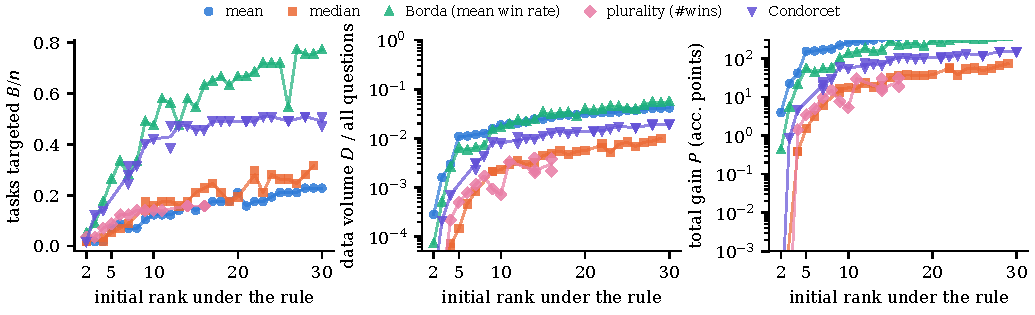
\includegraphics[width=\textwidth]{figs/fig_rank.pdf}
\caption{Exact minimal investment to reach first versus the target's initial rank under the same rule (HELM-MMLU, ceiling $u{=}1$). Points: individual models; lines: median per rank. Left: breadth as a fraction of the 57 subjects; middle: data volume as a fraction of all 14{,}042 test questions (log); right: total accuracy points gained (log).}\label{fig:rank}
\end{figure*}

\subsection{Away from the top, the rule sets the currency of the investment}
\Cref{fig:rank} and \cref{tab:same} show how investment grows with the initial distance.
\textbf{Additive rules are data-hungry.} Under the mean the median target ranked 4--10 must learn 168 questions (1.2\% of the benchmark) over 4 tasks, ranks 11--30 need 449 (3.2\%) over 10 tasks, and ranks $\ge31$ need 1{,}275 (9.1\%) over 21 tasks ($0.37n$). Under Borda the same groups need 91, 535 and 1{,}719 questions (12.2\% for the last), the latter over 51 of 57 tasks.
\textbf{Pivotal rules are cheap in data.} For ranks $\ge31$ the median rule needs 374 questions (2.7\%) over 26 tasks ($0.46n$), Condorcet 532 (3.8\%) over 29 tasks, plurality 92 (0.7\%) over 9 tasks.
\Cref{tab:paired} compares rules on the \emph{same} 78 targets: relative to the mean, median, Condorcet and plurality need 3.6$\times$, 2.1$\times$ and 10$\times$ less data (ratios of medians; all paired CIs exclude 0, Wilcoxon $p<10^{-7}$, though targets share rivals so $p$-values are indicative only), Borda needs more (+271 questions, CI [+180,+405]); in breadth the mean is cheapest except against plurality ($-7$ tasks).
The mechanism follows \cref{p:mean,p:quantile}: the mean charges for the \emph{whole} gap, wherever it is closed (and it is closed on the cheapest 100-question subjects), while the median/plurality/Condorcet charge only for crossing thresholds on pivotal tasks. Borda charges for every rival overtaken on every task, making it the most expensive in both currencies.
\Cref{tab:bins} gives the grouped medians; they are stable under evaluation noise (200 binomial replicates of the matrix, ranks recomputed: 95\% intervals e.g.\ mean, ranks 11--30: $B^\ast\in[9,11]$, $D^\ast\in[420,506]$; \cref{tab:noisebins}). Bounds are tight where predicted (\cref{tab:bounds}): $\Bst$ equals the closed form for the median (79/79 targets), the single-rival bound for Borda (78/78) and the Condorcet margin bound (78/78); no bound is ever violated, while the plurality bound (which ignores the coupling across rivals) and the mean bound are loose by 2 and 4 tasks at the median.

\begin{table}[t]
\caption{HELM-MMLU: investment by initial-rank group (median over target models; IQR of $B/n$). $D$ in questions (of 14{,}042); $P$ in accuracy points summed over tasks. Under plurality most models have no first place and tie, hence the uneven group sizes.}\label{tab:bins}
\centering\scriptsize\setlength{\tabcolsep}{2.5pt}
\begin{tabular}{@{}llrrrr@{}}\toprule
Rule & Initial ranks & \#models & $B/n$ med. [IQR] & $D$ (questions) & $P$ (acc. pts)\\\midrule
mean & 2-3 & 2 & 0.02 [0.02-0.02] & 13 & 13.2\\
 & 4-10 & 7 & 0.07 [0.07-0.10] & 168 & 167.5\\
 & 11-30 & 20 & 0.18 [0.16-0.21] & 449 & 434.8\\
 & 31-79 & 49 & 0.37 [0.28-0.44] & 1275 & 1021.4\\
\midrule
median & 2-3 & 2 & 0.02 [0.02-0.02] & 0 & 0.0\\
 & 4-10 & 8 & 0.08 [0.05-0.14] & 9 & 4.7\\
 & 11-30 & 19 & 0.23 [0.18-0.26] & 77 & 37.6\\
 & 31-79 & 50 & 0.46 [0.37-0.51] & 374 & 203.0\\
\midrule
Borda & 2-3 & 2 & 0.07 [0.06-0.08] & 4 & 3.0\\
 & 4-10 & 7 & 0.33 [0.27-0.40] & 91 & 55.1\\
 & 11-30 & 20 & 0.67 [0.58-0.72] & 535 & 285.8\\
 & 31-79 & 49 & 0.89 [0.84-0.93] & 1719 & 857.5\\
\midrule
plurality & 2-3 & 2 & 0.04 [0.04-0.04] & 0 & 0.0\\
 & 4-10 & 7 & 0.12 [0.11-0.14] & 11 & 5.3\\
 & 11-30 & 6 & 0.16 [0.16-0.16] & 39 & 24.2\\
 & 31-79 & 63 & 0.16 [0.16-0.16] & 92 & 58.1\\
\midrule
Condorcet & 2-3 & 2 & 0.07 [0.04-0.10] & 1 & 0.4\\
 & 4-10 & 7 & 0.32 [0.26-0.36] & 45 & 24.5\\
 & 11-30 & 20 & 0.49 [0.47-0.50] & 197 & 107.0\\
 & 31-79 & 49 & 0.51 [0.51-0.51] & 532 & 311.7\\
\bottomrule\end{tabular}

\end{table}
\begin{table}[t]
\caption{Tightness of the analytic bounds on $\Bst$ (HELM, ceiling): fraction of non-leader targets with equality, median excess, and violations.}\label{tab:bounds}
\centering\scriptsize
\begin{tabular}{@{}lrrrr@{}}\toprule
Rule & targets & violations & $B^\ast=$ bound & median $B^\ast-$bound\\\midrule
mean & 78 & 0 & 0.10 & 4\\
median & 79 & 0 & 1.00 & 0\\
borda & 78 & 0 & 1.00 & 0\\
plurality & 78 & 0 & 0.04 & 2\\
condorcet & 78 & 0 & 1.00 & 0\\
\bottomrule\end{tabular}

\end{table}
\begin{table*}[t]
\caption{Paired comparison with the mean on the same targets (non-leaders under both rules; 78, plurality 77): median breadth and data volume under the rule and under the mean, median paired difference with 95\% bootstrap CI, and fraction of targets for which the rule is cheaper/costlier.}\label{tab:paired}
\centering\small\setlength{\tabcolsep}{3pt}
\begin{tabular}{@{}lrrrrrrrr@{}}\toprule
 & \multicolumn{4}{c}{breadth $B^\ast$ (tasks)} & \multicolumn{4}{c}{data volume $D^\ast$ (questions)}\\
\cmidrule(lr){2-5}\cmidrule(lr){6-9}
Rule vs.\ mean & median & mean & diff [95\% CI] & cheaper/costlier & median & mean & diff [95\% CI] & cheaper/costlier\\\midrule
median & 21 & 16 & +4.0 [+3, +4] & 0.14/0.82 & 217 & 777 & -573 [-722, -451] & 1.00/0.00\\
Borda & 47 & 16 & +28.5 [+27, +29] & 0.00/1.00 & 1047 & 777 & +271 [+180, +405] & 0.12/0.88\\
plurality & 9 & 16 & -7.0 [-10, -4] & 0.81/0.14 & 79 & 824 & -743 [-961, -548] & 1.00/0.00\\
Condorcet & 29 & 16 & +12.0 [+9, +14] & 0.12/0.87 & 375 & 777 & -426 [-570, -312] & 1.00/0.00\\
\bottomrule\end{tabular}

\end{table*}

\subsection{The ordering of rules reverses under bounded gains or convex costs}\label{sec:convex}
The low breadth of the mean exploits unlimited headroom on a few tasks and constant marginal cost (A3, A4). \Cref{fig:caps} caps the gain per task at $g$ accuracy points.
For targets ranked 2--10 all rules are feasible once $g\ge5$ points, but with $g=2$ only 33\% of targets can reach first under the mean (Borda 44\%, median 70\%, plurality/Condorcet 78\%). For targets ranked $\ge11$, feasibility at $g=10$ is 29\% (mean), 22\% (Borda), 45\% (median), 42\% (Condorcet), 70\% (plurality), and the median breadth among feasible targets at $g=10$ is 44.5 of 57 tasks for the mean versus 16 (median), 28 (Condorcet), 9 (plurality) and 48 (Borda); only for $g\ge50$ points does the mean return to 17--18 tasks.
Convex costs act the same way (\cref{p:convex}; quadratic cost, closed forms): the cost-optimal mean plan spreads the gap over all 57 tasks (largest single-task gain 2.8 points for targets ranked 2--10, 14.6 for ranks $\ge11$), whereas the median plan needs 4 tasks (ranks 2--10) or 22 tasks (ranks $\ge11$) with at most 1.0 resp.\ 11.3 points on any task and a summed gain of 2 resp.\ 135 points against 156 resp.\ 768 for the mean (\cref{tab:convex}).
Hence ``the mean is the easiest rule to manipulate in breadth'' holds only when per-task gains are cheap and unbounded.

\begin{figure*}[t]
\centering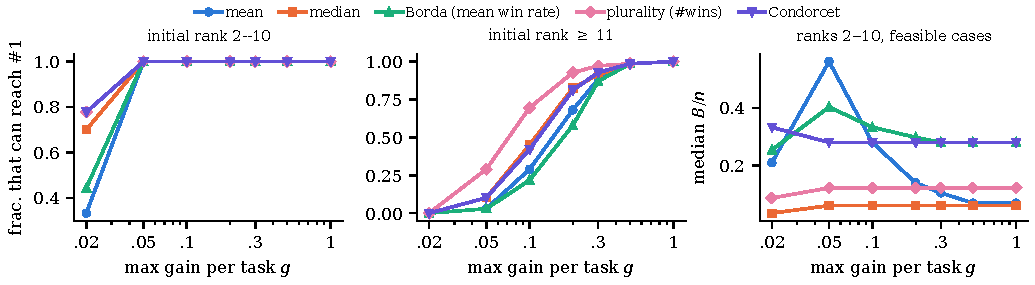
\includegraphics[width=\textwidth]{figs/fig_caps.pdf}
\caption{Bounded per-task gain $g$ (HELM). Left/middle: fraction of targets that can reach first; right: median breadth among feasible targets ranked 2--10.}\label{fig:caps}
\end{figure*}

\begin{table}[t]
\caption{Quadratic per-task cost (closed forms, HELM, ceiling): medians over targets of the breadth fraction, the summed gain and the largest single-task gain (accuracy points). Under the mean the cost-optimal plan touches every task.}\label{tab:convex}
\centering\scriptsize\setlength{\tabcolsep}{2.5pt}
\begin{tabular}{@{}llrrrr@{}}\toprule
Rule & ranks & \# & $B/n$ & $\sum_j\Delta_j$ & $\max_j\Delta_j$\\\midrule
mean & 2--10 & 9 & 1.00 & 156 & 2.8\\
mean & 11--79 & 69 & 1.00 & 768 & 14.6\\
median & 2--10 & 10 & 0.06 & 2 & 1.0\\
median & 11--79 & 69 & 0.39 & 135 & 11.3\\
\bottomrule\end{tabular}

\end{table}

\subsection{Scaling with the number of tasks, and noise}
We draw random subsets of the 57 subjects (60 per size, seed 0) and take the 6th-ranked model under each rule as target. The median total gain $P$ grows almost linearly in $n$ for the mean (log-log slope 0.98) and Borda (0.87), sublinearly for Condorcet (0.62), and is flat for plurality (0.15) and median (0.01) (\cref{fig:scale}): adding tasks raises the price of additive rules proportionally but not of pivotal rules.
Breadth grows roughly proportionally with $n$ for Borda and Condorcet ($B/n\approx0.25$--$0.33$ at $n{=}57$) and more slowly for the others ($B/n$ falls from 0.14--0.29 at $n{=}7$ to 0.07--0.12 at $n{=}57$ for mean, median and plurality).

\begin{figure}[t]
\centering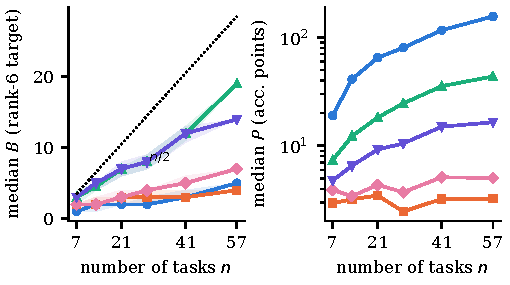
\includegraphics[width=\columnwidth]{figs/fig_scale.pdf}
\caption{Scaling with the number of subsets $n$ (median and IQR over 60 random subsets; target = 6th-ranked model). Dotted: $n/2$.}\label{fig:scale}
\end{figure}
\begin{figure*}[t]
\centering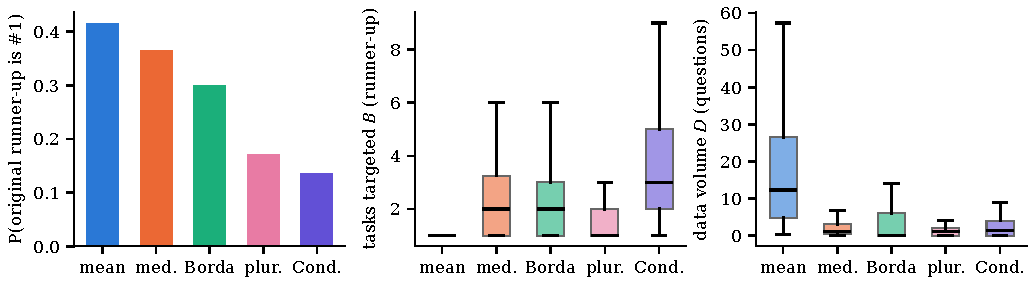
\includegraphics[width=\textwidth]{figs/fig_noise.pdf}
\caption{Evaluation-noise bootstrap (200 replicates). Left: probability that the original runner-up is first in a resampled leaderboard. Middle/right: breadth and data volume the runner-up of each replicate needs.}\label{fig:noise}
\end{figure*}

\subsection{A second leaderboard: Open LLM Leaderboard (n = 6)}
With six tasks breadth is trivially small (at ceiling, $\Bst\le3$ for all 21 top targets of the full board under every rule) and the informative quantity is the \emph{size} of the gain.
Targets ranked 6--11 under the mean need a median of 28 normalised points on one task under the mean, but 0.6 (median rule), 7.3 (Borda), 12.8 (Condorcet, 2--3 tasks) and 18.9 points (plurality, 2 tasks); with realistic caps the pivotal rules become the \emph{hardest}: for $g=5$ points only 15\% (plurality) and 30\% (Condorcet) of the top-21 models on the full board can reach first versus 65\% (mean) and 75\% (median, Borda) (\cref{fig:olb}). Winning a task outright requires beating specialised leaders by wide margins, unlike HELM-MMLU where the top of each subject is tightly packed.
On the official-provider board (470 models) the median rule is the hardest at small $g$ (10\% feasible at $g=5$, 25\% at $g=10$).
The ordering of rules is thus board-specific.

\begin{figure*}[t]
\centering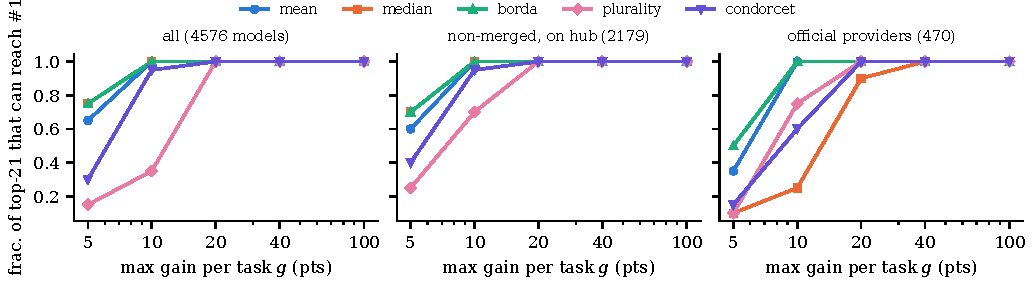
\includegraphics[width=\textwidth]{figs/fig_olb.pdf}
\caption{Open LLM Leaderboard: fraction of the top-21 models (by the official mean) that can reach first when each task can gain at most $g$ normalised points, for three board variants.}\label{fig:olb}
\end{figure*}

\subsection{Ablations}
\textbf{Informed vs.\ random task choice.} Lifting tasks to the ceiling in uniformly random order needs 1.78$\times$ the optimal breadth for the mean (IQR 1.51--2.10), 1.16$\times$ median, 1.23$\times$ plurality, 1.09$\times$ Borda and 1.00$\times$ Condorcet (\cref{tab:random}): knowing the leaderboard matters mostly under additive rules with heterogeneous headroom. \textbf{Cost currency.} Optimising data instead of points changes which tasks are targeted: the runner-up's data-optimal mean plan puts its 4.0 points on a 100-question subject ($D^\ast=4.0$ questions for $P^\ast=4.0$ points), whereas the average subject has 246 questions.

\begin{table}[t]
\caption{Informed versus random task choice (HELM, ceiling): tasks lifted to the ceiling in random order until the target is first (20 permutations per target, fixed seeds).}\label{tab:random}
\centering\scriptsize\setlength{\tabcolsep}{2.5pt}
\begin{tabular}{@{}lrrrr@{}}\toprule
Rule & targets & $B^\ast$ (optimal) & $B$ random order & ratio, median [IQR]\\\midrule
borda & 78 & 47 & 51.2 & 1.09 [1.03, 1.24]\\
condorcet & 78 & 29 & 29.0 & 1.00 [1.00, 1.03]\\
mean & 78 & 16 & 28.3 & 1.78 [1.51, 2.10]\\
median & 79 & 21 & 24.3 & 1.16 [1.03, 1.38]\\
plurality & 78 & 9 & 11.1 & 1.23 [1.22, 1.26]\\
\bottomrule\end{tabular}

\end{table}

\section{Discussion and Limitations}\label{sec:disc}
\textbf{What we expected and what we found.} Before running the experiments we expected the median to be markedly more robust (needing about half of the tasks, \cref{p:quantile}). This holds only for targets far from the top ($0.46n$ for ranks $\ge31$): the 10 closest contenders need $0.06$--$0.08\,n$ because they already exceed the leader's median on many tasks ($a$ large); the quantile family shows no monotone relation between the statistic's position and the required breadth (\cref{fig:quantile}). We also expected pivotal rules to be uniformly cheaper; on the Open LLM Leaderboard with realistic caps they are the hardest.
\textbf{Answer.} On these leaderboards, topping the board requires (i) almost nothing near the top, where differences are a handful of test questions and below evaluation noise; (ii) away from the top, an amount that is set by the rule: data volume proportional to the gap for additive rules, a count of pivotal tasks for median/plurality/Condorcet; (iii) a form that depends on headroom and cost curvature: concentrated and deep if gains are cheap and unbounded, spread over most tasks otherwise. We do \emph{not} find that any rule is robust in general: \cref{p:sep} and the OLB/HELM contrast show that the preferred rule depends on the board's score structure.
\begin{table*}[t]
\caption{Testable claims, the evidence in this paper, and their scope.}\label{tab:claims}
\centering\scriptsize\setlength{\tabcolsep}{3pt}
\begin{tabular}{@{}p{4.6cm}p{3.2cm}p{4.2cm}p{4.8cm}@{}}\toprule
Claim & Evidence & Holds when & Fails / not tested when\\\midrule
C1. The two closest contenders (ranks 2--3) reach first with $\le4$ tasks and $\lesssim0.1\%$ of the benchmark's questions under every rule & Tab.~\ref{tab:same}, Fig.~\ref{fig:rank}, Tab.~\ref{tab:bins} (ranks 2--3) & HELM-MMLU, per-task gain $\ge5$ points & ranks $\ge4$ (mean: 168+ questions); gain $\le2$ points: 22--67\% of the top-10 cannot win (Fig.~\ref{fig:caps})\\
C2. These gaps are inside evaluation noise & Fig.~\ref{fig:noise}: runner-up is first in 13.5--41.5\% of resamples & independent binomial cell noise & correlated noise across tasks/models (not modelled)\\
C3. Additive rules (mean, Borda) need 2--13$\times$ more data than pivotal rules & Tab.~\ref{tab:paired} (78 paired targets) & linear cost, HELM $n{=}57$ & per-task gain caps in OLB: pivotal rules hardest (Fig.~\ref{fig:olb})\\
C4. The mean needs the fewest tasks & Tab.~\ref{tab:paired}, Fig.~\ref{fig:rank} & unbounded gains, linear cost & $g\le30$ points, convex cost (Fig.~\ref{fig:caps}, Tab.~\ref{tab:convex}); plurality is cheaper even then\\
C5. Median needs about half of the tasks & Prop.~\ref{p:quantile}; $0.46n$ for ranks $\ge31$ & target far from the top ($a$ small) & near-top contenders ($0.06$--$0.08n$)\\
C6. Total gain grows $\propto n$ for additive rules, not for pivotal rules & Fig.~\ref{fig:scale} (slopes 0.98, 0.87 vs 0.01, 0.15) & random subsets of HELM subjects; 6th-ranked target & other boards, other targets: not tested\\
\bottomrule\end{tabular}
\end{table*}
\textbf{Implications.} Fixing the rule cannot protect a dense leaderboard top; reporting uncertainty (ties within noise) can. Adding tasks raises the cost of additive rules linearly but does not help pivotal ones (\cref{fig:scale}).
\textbf{Limitations.} (1) A1--A3 favour the attacker: real training on task data spills over to related tasks (which would lower breadth further) but needs far more than one example per answer; $D$ is thus a lower bound under a ``leak'' pathway and cross-rule \emph{ratios} are more reliable than absolute values. (2) One-shot static rivals: no competitor response, no multiple targets, no designer reaction. (3) Rank 1 is strict; ties (frequent in 100-question subjects) make some zero-cost entries (e.g.\ median) artefacts of exact ties, which the noise analysis shows. (4) Costs are exact optima within the model but the plurality bound is loose and MILP optimality is tolerance-based (all runs reported status optimal). (5) We analyse two boards and one HELM release; subjects are correlated and the noise model treats cells as independent. (6) Ceilings at 1 are unrealistic for MMLU (label noise); that is why we report $g$-sweeps. (7) Ties at a ceiling are ignored; no cell in either board equals 1.0. (8) The bootstrap treats observed scores as truth. (9) We do not train any model, so how much real data a given gain needs is not measured.

\section*{Impact Statement}
This paper analyses how aggregation rules price strategic training on benchmark-related data. It may help designers choose and audit rules; it also describes what a manipulator would need, but uses only public numbers and cannot itself be used to train or deploy a model.

\bibliography{refs}
\bibliographystyle{icml2026}

\newpage
\appendix
\onecolumn
\section{Proofs}\label{app:proofs}
Throughout, $\Delta_j=x_j-s_j\ge0$, $h_j=u_j-s_j\ge0$.

\paragraph{Proof of \cref{p:mean}.}
$t$ is first iff $\sum_jx_j>\max_{i\ne t}\sum_jS_{ij}$, i.e.\ $\sum_j\Delta_j>G$. Since $\sum_j\Delta_j\le\sum_jh_j$, the plan exists iff $\sum_jh_j>G$. Every plan with total gain $>G$ is feasible, so $\inf\sum_j\Delta_j=G$ (not attained). Touching $k$ tasks yields at most the sum of the $k$ largest headrooms, which must exceed $G$; filling the largest headrooms first attains it, giving $\Bst$ and $\Bst\ge G/\max_jh_j$. For $D$ the problem is $\min\sum_jN_j\Delta_j$ s.t.\ $\sum_j\Delta_j>G$, $0\le\Delta_j\le h_j$, a fractional knapsack whose optimum fills tasks in increasing $N_j$. \qed

\paragraph{Proof of \cref{p:quantile}.}
$f_r(x)>\theta$ iff at least $r$ coordinates of $x$ exceed $\theta$. Initially $a$ do. Raising a coordinate that already exceeds $\theta$ does not change the count and raising one that does not can increase it by one only if it is pushed above $\theta$, which needs $u_j>\theta$. So at least $r-a$ coordinates with $s_j\le\theta$ must be touched (fewer touches leave the count $\le r-1$, hence $f_r\le\theta$), and $r-a$ suffice when enough eligible tasks exist; each is raised to $\theta+\epsilon$ at cost $w_j(\theta-s_j+\epsilon)$ and the cheapest $r-a$ are chosen. Beating $\theta=\max_i f_r(S_i)$ is equivalent to beating every rival. \qed

\paragraph{Proof of \cref{p:margin}.}
For rival $i$ let $M_i(x)=M_i(s)+\sum_j\phi_{ij}(x_j)$ with $\phi_{ij}$ non-decreasing, $\phi_{ij}(s_j)=0$ (the margin is a sum over tasks of terms in which only $x_j$ varies, and raising $x_j$ can only turn a loss into a tie/win or a tie into a win). Let $\gamma_{ij}=\phi_{ij}(u_j)$ be the maximal gain. Any plan that beats rival $i$ must satisfy $\sum_j\phi_{ij}(x_j)>-M_i(s)$ hence touch at least as many tasks as the shortest prefix of the $\gamma_{i\cdot}$ sorted decreasingly that exceeds $-M_i(s)$; this is $\Bst_i$ (attained for the single rival by lifting to the ceiling). A plan for the full problem beats all rivals, so $\Bst\ge\max_i\Bst_i$. The per-task bounds: for Condorcet $\phi_{ij}\le\mathrm{sign}(1)-\mathrm{sign}(-1)=2$; for plurality $t$ gains at most one win and $i$ loses at most one, so the margin changes by $\le2$; for Borda $t$ gains at most $m-1$ points on a task and $i$ loses at most one. \qed

\paragraph{Proof of \cref{p:sep}.}
(a) One rival with scores $0.5$ everywhere; target $0.5-\delta$ everywhere, $\delta=\frac{1}{4(n-1)}$. Mean: $G=n\delta<0.5+\delta=h_j$ for all $j$ (equivalent to $(n-1)\delta<0.5$), so one task suffices. Median: $\theta=0.5$, $a=0$, $r=\frac{n+1}2$, hence $\Bst=\frac{n+1}{2}$ by \cref{p:quantile}.
(b) Rival $0.5$ everywhere; target: $k=\frac{n-1}2$ tasks at $0.51$, one task at $0.49$, the other $k$ tasks at $0$. Then $a=k$ and $\Bst_{\text{median}}=r-a=1$ (lift the $0.49$ task). The mean gap is $G=\frac n2-0.51k-0.49=0.245n-0.235$, the $k$ zero tasks have headroom 1 (the largest), so $\Bst_{\text{mean}}=\lfloor G\rfloor+1=\lfloor 0.245n-0.235\rfloor+1$ whenever $G<k$. Both instances are verified numerically for $n\in\{5,9,21,57\}$ in \texttt{src/analysis\_theory.py} (output in \texttt{out/theory\_summary.txt}). \qed

\paragraph{Proof of \cref{p:convex}.}
The mean problem is $\min\sum_jc(\Delta_j)$ s.t.\ $\sum_j\Delta_j\ge G$, $0\le\Delta_j\le h_j$. It is strictly convex with a unique solution; KKT gives a multiplier $\lambda>0$ ($G>0$) with $c'(\Delta_j)=\lambda$ whenever $0<\Delta_j<h_j$, $c'(\Delta_j)\le\lambda$ if $\Delta_j=0$. Since $c'(0)=0<\lambda$, $\Delta_j=0$ with $h_j>0$ would contradict stationarity (raising $\Delta_j$ lowers the Lagrangian). Hence $\Delta_j>0$ for every $j$ with $h_j>0$; for $c(\Delta)=\Delta^2$ the solution is $\Delta_j=\min(h_j,\lambda/2)$. For order statistics, each pushed task must reach $\theta$ whatever the convexity, and an increasing $c$ makes the $r-a$ smallest gaps optimal. \qed

\section{Solvers and validation}\label{app:val}
\textbf{0--1 program.} For Borda, plurality and Condorcet and a target $t$, a rival is \emph{binding} if its margin over $t$ is $\le0$ (margins never decrease, so non-binding rivals stay beaten). Variables $y_{jl}\in\{0,1\}$ select for task $j$ a \emph{level} $v_{jl}$: the distinct rival scores in $[s_j,u_j)$ (placing $t$ at $v+\epsilon$ beats exactly the rivals with score $\le v$); for plurality the only level is just above the column maximum. Constraints: $\sum_ly_{jl}\le1$; for each binding rival $i$, $\sum_{jl}\mathrm{inc}_{i,jl}y_{jl}\ge\mathrm{need}_i$, where $\mathrm{inc}$ is the exact change in margin (for Borda the change in $t$'s points plus the loss of $i$'s points on that task; doubled so that half-points are integral). Objectives: $\sum y$ (breadth), $\sum(v-s_j)y$ (points) and $\sum N_j(v-s_j)y$ (data). HiGHS (via SciPy) is run with relative gap $10^{-9}$ and a 120\,s limit; the status of every solve is stored in the output CSVs (all runs terminated with status 0 = optimal; check with \texttt{grep} on the \texttt{status} column). Plurality shares are fractions, so rows are scaled by $10^4$ and require margin $\ge10^{-4}$ (conservative for margins below $10^{-4}$, which do not occur).
\textbf{Verification.} After solving, each of the three plans is applied to the leaderboard and the rule is recomputed from scratch; the code asserts that the target is strictly first (tolerance $10^{-11}$), $x\ge s$ and $x\le\max(u,s)$.
\textbf{Brute-force test} (\texttt{tests/test\_core.py}; output \texttt{out/test\_log.txt}): 300 random instances ($m{=}6$, $n{=}5$, scores on a 0.1 grid so ties are frequent, random continuous ceilings, random weights) for mean, median, $f_1,f_2,f_5$, Borda, plurality, Condorcet: $\Bst$ equals exhaustive search over subsets lifted to ceilings in every feasible case (feasibility also agrees), and $\Pst$, $\Dst$ equal exhaustive search over candidate levels (for the mean, $\Pst=G$). 100 instances for the even-$n$ median.
\textbf{Ties at ceilings.} A plan may place $t$ exactly at a rival's score (a tie) only at a ceiling; the solvers ignore such ties (conservative). No cell of either board equals 1, and caps $s_j+g$ are continuous.
\textbf{Even-$n$ median.} For $n=2k$ the median is the average of the $k$-th and $(k{+}1)$-th largest; $t$ wins iff $d_k+d_{k+1}>2M$. We enumerate the $k$-subset lifted to level $\alpha$ and one further task lifted to $2M-\alpha$ over all breakpoints $\alpha$ (exact for small $n$); breadth by subset enumeration.

\section{Additional results}\label{app:extra}
\begin{table}[h]
\caption{Open LLM Leaderboard (all 4{,}576 models), top-21 targets by the official mean: feasibility (fraction reaching first) and median breadth among all targets (infeasible ones counted as missing) at three per-task gain caps $g$ in normalised points.}
\centering\small\begin{tabular}{@{}lrrrrrr@{}}\toprule
 & \multicolumn{2}{c}{$g=5$} & \multicolumn{2}{c}{$g=20$} & \multicolumn{2}{c}{$g=100$ (ceiling)}\\
 Rule & feas. & $B$ & feas. & $B$ & feas. & $B$\\\midrule
mean & 0.65 & 6 & 1.00 & 2 & 1.00 & 1\\
median & 0.75 & 1 & 1.00 & 1 & 1.00 & 1\\
borda & 0.75 & 2 & 1.00 & 1 & 1.00 & 1\\
plurality & 0.15 & 2 & 1.00 & 2 & 1.00 & 2\\
condorcet & 0.30 & 3 & 1.00 & 3 & 1.00 & 3\\
\bottomrule\end{tabular}

\end{table}
\begin{table}[h]
\caption{Stability of rank-group medians under evaluation noise (200 binomial replicates, seed 4; ranks recomputed in each replicate).}\label{tab:noisebins}
\centering\small\begin{tabular}{@{}llrr@{}}\toprule
Rule & ranks & $B^\ast$ median [95\% interval] & $D^\ast$ median [95\% interval]\\\midrule
mean & 4-10 & 5.0 [4.0, 6.0] & 178 [142, 220]\\
mean & 11-30 & 10.0 [9.0, 11.0] & 455 [420, 506]\\
mean & 31-79 & 21.0 [20.0, 22.0] & 1276 [1208, 1342]\\
median & 4-10 & 6.5 [3.5, 10.0] & 15 [5, 35]\\
median & 11-30 & 14.0 [12.0, 17.0] & 89 [65, 119]\\
median & 31-79 & 26.0 [25.0, 27.0] & 392 [348, 450]\\
\bottomrule\end{tabular}

\end{table}
\begin{figure}[h]
\centering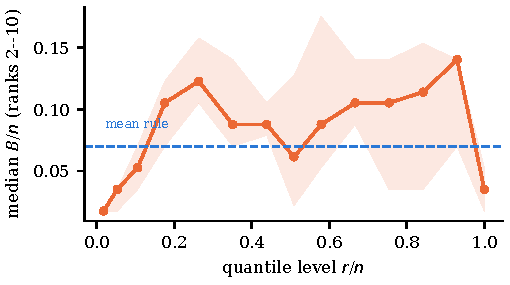
\includegraphics[width=.5\textwidth]{figs/fig_quantile.pdf}
\caption{Order-statistic family on HELM (ceiling): median $B/n$ over targets with initial rank 2--10 versus quantile level $r/n$ ($r$-th largest score; $r/n=1/57$ is the maximum, 0.51 the median, 1 the minimum). Band: IQR. Dashed: mean rule. Breadth is not monotone in $r$: near the top it is governed by $a$ in \cref{p:quantile}, not by the position of the statistic.}\label{fig:quantile}
\end{figure}

\section{Reproducibility}\label{app:repro}
\textbf{Code and data.} Everything is in the supplementary directory: \texttt{src/} (library \texttt{core.py}, experiments \texttt{exp\_*.py}, analysis \texttt{analysis\_*.py}), \texttt{tests/}, \texttt{run\_all.sh}, \texttt{README.md} (environment, commands, runtimes). Data are downloaded by \texttt{src/download\_data.py} (no account required); \texttt{data/CHECKSUMS.sha256} lists sha256 of all 304 files (HELM release v1.13.0: 303 files; OLB parquet sha256 \texttt{f13a7061\ldots dca5}). Python 3.11.2, numpy 2.4.6, scipy 1.17.1 (HiGHS), pandas 3.1.0, pyarrow 26.0.0, matplotlib 3.11.2.
\textbf{Seeds.} Task subsets seed 0 (Exp.\ C), noise bootstrap seed 1 (D), random permutations seeds $1000i+t$ for rule index $i$ and target $t$ (G), paired bootstrap seed 3. All solvers are deterministic.
\textbf{Licences.} HELM code is Apache-2.0; no separate licence is stated for the bucket's score data; the OLB \texttt{contents} dataset card has no licence field (it lists each model's hub licence). We use only the numeric scores and model names, redistribute no data (scripts download them), and cite the sources.
\textbf{Version choice.} HELM v1.13.0 is the version prescribed in the task and is the only version used.
\textbf{Scripts per artefact.} \cref{fig:rank} (Fig.\ 1), Tab.\ 1--2, \cref{tab:paired}: \texttt{exp\_helm\_main.py}+\texttt{analysis\_helm.py}; \cref{fig:caps}: \texttt{exp\_helm\_caps.py}; \cref{fig:scale}: \texttt{exp\_helm\_scale.py}; \cref{fig:noise}: \texttt{exp\_helm\_noise.py}; quantile figure: \texttt{exp\_helm\_quantile.py}; random ablation: \texttt{exp\_helm\_random.py}; convex table: \texttt{exp\_helm\_convex.py}; \cref{fig:olb} and OLB table: \texttt{exp\_olb.py}+\texttt{analysis\_olb.py}; bound table, separation instances: \texttt{analysis\_theory.py}; all figures/tables are rewritten by \texttt{run\_all.sh}.
\textbf{Access to restricted material.} The task forbids reading a specific published paper and derivative pages. Searches (scholarly-search tool) used the queries: bribery in elections; margin of victory in elections; robustness of benchmark rankings to task selection; Goodhart's law leaderboards; training on the test task; diversity--stability in benchmarks; computational social choice handbook; Open LLM Leaderboard contamination. Result lists were read as title/abstract snippets only; none was identified as the restricted paper or a page discussing it. The only item in the lists on strategic post-training is the starter-list reference \cite{chen2026leaderboard}, of which only the search-result abstract snippet was read.

\end{document}
